\documentclass{beamer}
%~ \documentclass[hyperref={pdfpagelabels=false}]{beamer}

\usepackage[ngerman,english]{babel}
\usepackage[utf8]{inputenc}
\usepackage{lmodern}
\usepackage{beamerthemeshadow}

\usepackage{mdframed}

%\usepackage{la}
\usepackage[T1]{fontenc}

\definecolor{mygreen}{rgb}{0,0.5,0}
\usecolortheme[named=mygreen]{structure}

\usepackage{listings}
\lstdefinestyle{sharpc}{language=[Sharp]C, frame=lr, rulecolor=\color{blue!80!black}}

\title{A Unified Image Processing Framework\\for Computer Vision and Remote Sensing}
\author{
Carsten Brandt,
Ludmilla Brandt,
Marcus Zepp,\\
Akarsh Seggemu
}
\date{July 15, 2015}

\newcommand{\beginbackup}{
   \newcounter{framenumbervorappendix}
   \setcounter{framenumbervorappendix}{\value{framenumber}}
}
\newcommand{\backupend}{
   \addtocounter{framenumbervorappendix}{-\value{framenumber}}
   \addtocounter{framenumber}{\value{framenumbervorappendix}}
}

% table of contents should not show subsections
\setcounter{tocdepth}{1}

% allow using color
\usepackage{color}
\usepackage{xcolor}

% the lstlistings package
\usepackage{listings}
% highlighting lines in listings
\usepackage{linehighlight}

% set colors for code background and highlighting
\definecolor{codehighlight}{rgb}{0.95,0.8,0.8}
\definecolor{codebackground}{rgb}{0.95,0.95,0.95}

%~ % Dadurch wird verhindert, dass die Navigationsleiste angezeigt wird.
%~ \setbeamertemplate{navigation symbols}{}
\setbeamertemplate{footline}{
  \leavevmode%
  \hbox{%
	  \begin{beamercolorbox}[wd=.75\paperwidth,ht=2.25ex,dp=1ex,center]{author in head/foot}%
			\usebeamerfont{author in head/foot}\insertshortauthor%~~(\insertshortinstitute)
	  \end{beamercolorbox}%
%	  \begin{beamercolorbox}[wd=.5\paperwidth,ht=2.25ex,dp=1ex,center]{title in head/foot}%
%			\usebeamerfont{title in head/foot}\insertshorttitle
%	  \end{beamercolorbox}%
	  \begin{beamercolorbox}[wd=.25\paperwidth,ht=2.25ex,dp=1ex,right]{date in head/foot}%
			\usebeamerfont{date in head/foot}\insertshortdate{}\hspace*{2em}
			\insertframenumber{} / \inserttotalframenumber % hier hat's sich geändert
	  \end{beamercolorbox}
	  }%
  \vskip0pt%
}

% http://tex.stackexchange.com/questions/16357/how-can-i-position-an-image-in-an-arbitrary-position-in-beamer
\usepackage{tikz}
%\usetikzlibrary{calc, trees, positioning, arrows, shapes, shapes.multipart, shadows, matrix, decorations.pathreplacing, decorations.pathmorphing}
\usetikzlibrary{arrows}%, shapes, shapes.multipart}

% creating histograms
% http://tex.stackexchange.com/questions/130531/automatic-binning-of-histogram-using-raw-gnuplot-in-pgfplot
% \usepackage{pgfplots}
% \usepackage{pgfplotstable}
% \usetikzlibrary{external}
% \tikzexternalize
% \tikzset{external/force remake}
% %\pgfplotsset{compat=1.8}


\tikzset{
  every boverlay node/.style={
    draw=black,fill=white,rounded corners,anchor=north west,
  },
}
\tikzset{
  every overlay node/.style={
    %draw=white,fill=white,rounded corners,anchor=north west,
    anchor=north west
  },
}
% Usage:
% \tikzoverlay at (-1cm,-5cm) {content};
% or
% \tikzoverlay[text width=5cm] at (-1cm,-5cm) {content};
\def\tikzboverlay{%
   \tikz[baseline,overlay]\node[every boverlay node]
}%
\def\tikzoverlay{%
   \tikz[baseline,overlay]\node[every overlay node]
}%

\usetheme{default}
% default, bars, boxes, classic, lined, plain, shadow, sidebar, split, tree
% Berlin, Darmstadt, Dresden, Frankfurt, Goettingen, Hannover, Ilmenau, Luebeck, . . . , Warsaw

\usepackage{pdfpcnotes}

% Notizen zu jeder Folie auf zweitem Bildschirm anzeigen
%~ \setbeameroption{show notes on second screen = right}
% Notizen beliebig innerhalb des Frames setzen:
% 1 (...)
% 2 \note{Hier eine Notiz}
% 3 (...)
% 4 \note[item]{und noch eine Notiz , diesmal geordnet}
% 5 (...)



\definecolor{codehighlight}{rgb}{0.95,0.8,0.8}
\definecolor{codebackground}{rgb}{0.95,0.95,0.95}

\definecolor{exercisecolor}{rgb}{0.63, 0.90, 1.00}

\definecolor{lightgrey}{rgb}{0.9,0.9,0.9}
\definecolor{mygreen}{rgb}{0,0.6,0}
\definecolor{mygray}{rgb}{0.5,0.5,0.5}
\definecolor{mymauve}{rgb}{0.58,0,0.82}

\lstset{ %
%	backgroundcolor=\color{lightgrey},   % choose the background color; you must add \usepackage{color} or \usepackage{xcolor}
	breakatwhitespace=true,          % sets if automatic breaks should only happen at whitespace
	breaklines=true,                 % sets automatic line breaking
	captionpos=b,                    % sets the caption-position to bottom
%	deletekeywords={...},            % if you want to delete keywords from the given language
%	escapeinside={\%*}{*)},          % if you want to add LaTeX within your code
%	extendedchars=true,              % lets you use non-ASCII characters; for 8-bits encodings only, does not work with UTF-8
	frame=single,                    % adds a frame around the code
	keepspaces=true,                 % keeps spaces in text, useful for keeping indentation of code (possibly needs columns=flexible)
	language=C++,                    % the language of the code
	morekeywords={*,php,class,extends,public,protected,private,foreach,if,else,elseif,%
		function,return,new,echo,endforeach,vector,Context
	},            % if you want to add more keywords to the set
	numbers=left,                    % where to put the line-numbers; possible values are (none, left, right)
	numbersep=10pt,                   % how far the line-numbers are from the code
%	rulecolor=\color{black},         % if not set, the frame-color may be changed on line-breaks within not-black text (e.g. comments (green here))
	showspaces=false,                % show spaces everywhere adding particular underscores; it overrides 'showstringspaces'
	showstringspaces=false,          % underline spaces within strings only
	showtabs=false,                  % show tabs within strings adding particular underscores
	stepnumber=1,                    % the step between two line-numbers. If it's 1, each line will be numbered
	tabsize=4,                       % sets default tabsize to 2 spaces
%	title=\lstname                   % show the filename of files included with \lstinputlisting; also try caption instead of title
	basicstyle=\footnotesize\ttfamily,
	keywordstyle=\bfseries\color{green!40!black},
	commentstyle=\color{purple!40!black},
	identifierstyle=\color{black},
	stringstyle=\color{orange},
	numberstyle=\tiny\color{mygray}, % the style that is used for the line-numbers
}

% A language definition to highlight YAML code:
% http://tex.stackexchange.com/questions/152829/how-can-i-highlight-yaml-code-in-a-pretty-way-with-listings
\newcommand\YAMLcolonstyle{\color{red}\mdseries}
\newcommand\YAMLkeystyle{\color{black}\bfseries}
\newcommand\YAMLvaluestyle{\color{blue}\mdseries}

\makeatletter

% here is a macro expanding to the name of the language
% (handy if you decide to change it further down the road)
\newcommand\language@yaml{yaml}

\expandafter\expandafter\expandafter\lstdefinelanguage
\expandafter{\language@yaml}
{
  keywords={true,false,null,y,n},
  keywordstyle=\color{darkgray}\bfseries,
  basicstyle=\YAMLkeystyle,                                 % assuming a key comes first
  sensitive=false,
  comment=[l]{\#},
  morecomment=[s]{/*}{*/},
  commentstyle=\color{purple}\ttfamily,
  stringstyle=\YAMLvaluestyle\ttfamily,
  moredelim=[l][\color{orange}]{\&},
  moredelim=[l][\color{magenta}]{*},
  moredelim=**[il][\YAMLcolonstyle{:}\YAMLvaluestyle]{:},   % switch to value style at :
  morestring=[b]',
  morestring=[b]",
  literate =    {---}{{\ProcessThreeDashes}}3
                {>}{{\textcolor{red}\textgreater}}1
                {|}{{\textcolor{red}\textbar}}1
                {\ -\ }{{\mdseries\ -\ }}3,
}

% switch to key style at EOL
\lst@AddToHook{EveryLine}{\ifx\lst@language\language@yaml\YAMLkeystyle\fi}
\makeatother

\newcommand\ProcessThreeDashes{\llap{\color{cyan}\mdseries-{-}-}}



%  \beamersetuncovermixins{\opaqueness<1>{25}}{\opaqueness<2->{15}}
%  sorgt dafuer das die Elemente die erst noch (zukuenftig) kommen
%  nur schwach angedeutet erscheinen
\beamersetuncovermixins{\opaqueness<1>{25}}{\opaqueness<2->{15}}
% klappt auch bei Tabellen, wenn teTeX verwendet wird\ldots

\begin{document}


\begin{frame}
	\titlepage
\end{frame}

\begin{frame}
	\tableofcontents  \pnote{}
\end{frame}

% Vor jedem Abschnitt automatisch Inhaltsverzeichnis anzeigen:
\AtBeginSection []{
\begin{frame}
	\tableofcontents [currentsection]

	%~ \pnote{
		%~ notes go here...
	%~ }
\end{frame}
}

%---------------------------------------------------------------------------------------------------------------------------------------------

%%%%%%%%%%%%%%%%%%%%%%%%%%% part 1:  Mila %%%%%%%%%%%%%%%%%%%%%%%%%%%%%%%%%%%%%%%%%%%%%%%%%%%%%%
\section{What is this all about?}
\begin{frame}[t]{Unified Image Processing Framework}
\begin{center}
\begin{tikzpicture}
	\node<1-> [] (in) at (0,0) {Input};
	\node<1-> []  at (4,-1) {Program};
	\node<1-> []  at (4,0.4) {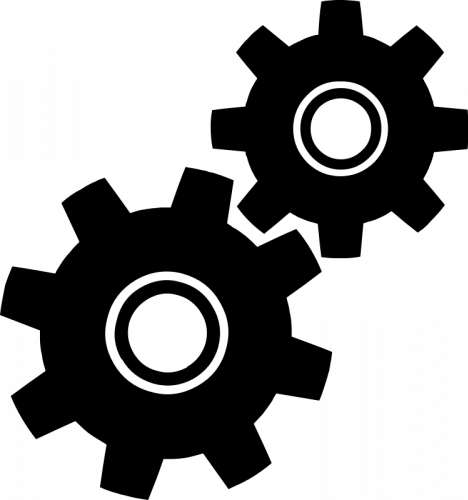
\includegraphics[scale=0.1]{images/wheels}};
	\node<1-> [draw,shape=rectangle,rounded corners,minimum width=3cm,minimum height=3cm] (pr) at (4,0) {};
	\node<1-> [] (out) at (8,0) {Output};
	\draw<1-3> [blue, ->, thick] (in) -- (pr);
	\draw<1-3> [blue, ->, thick] (pr) -- (out);
	\node<2-> [] (m1) at (2,-3) {module};
	\node<2-> [] (m2) at (4,-3) {module};
	\node<2-> [] (m3) at (6,-3) {module};
	\draw<2-> [mygreen, ->, thick] (pr) -- (m1);
	\draw<2-> [mygreen, ->, thick] (pr) -- (m2);
	\draw<2-> [mygreen, ->, thick] (pr) -- (m3);
	\draw<3-> [gray, <->, thick] (m1) -- (m2);
	\draw<3-> [gray, <->, thick] (m2) -- (m3);
	\draw<4> [red, ->, thick] (in) -- (m1);
	\draw<4> [red, ->, thick] (m3) -- (out);
\end{tikzpicture}
\end{center}

\pnote{
	usual workflow\\
	split your program in many methods\\
	each method is self contained - called module\\
	e.g. load, gaussian, store\\
	modules interact with each other\\
	program is replaced by the chain of modules\\
	get same results
}

\end{frame}

\begin{frame}{Use given modules}
	\begin{mdframed}[backgroundcolor=red!20]
	Framework
	\begin{itemize}
		\item[-] module 1
		\item[-] module 2
		\item[]  $ \quad \vdots$
		\item[-] module n
	\end{itemize}
	\end{mdframed}
\pnote{
	framework already provides a list of modules\\
	if program consists only of given modules,...
}
\end{frame}

\begin{frame}{Specify execution order}
	\begin{mdframed}[backgroundcolor=green!20]
	Chain
	\begin{itemize}
		\item[] {\color{mygreen} step 1:} module 1
		\item[] {\color{mygreen} step 2:} module 2
		\item[] {\color{mygreen} step 3:} module 7
		\item[] {\color{mygreen} step 4:} module 13
	\end{itemize}
	\end{mdframed}

\begin{tikzpicture}[overlay]
	\draw [blue, ->, thick] (4,2.5) arc (90:-90:9pt);
	\draw [blue, ->, thick] (4.2,1.3) arc (90:-90:9pt);
	\draw [blue, ->, thick] (4,2.5) arc (90:-90:16pt);
	\draw [blue, ->, thick] (4.2,1.8) arc (90:-90:16pt);
	\node at (6.2,1.7) [blue, thick] {dependencies};
\end{tikzpicture}

\pnote{
	... just order them\\
	add dependencies and parameters\\
	you are finished
}

\end{frame}

\begin{frame}{Modify the chain}

\only<1>{
	\begin{mdframed}[backgroundcolor=green!20]
	Chain 1
	\begin{itemize}
		\item[] {\color{mygreen} step 1:} module 1
		\item[] {\color{mygreen} step 2:} module 2
		\item[] {\color{mygreen} step 3:} {\color{red} module 7}
		\item[] {\color{mygreen} step 4:} module 13
	\end{itemize}
	\end{mdframed}
}

\only<2>{
	\begin{mdframed}[backgroundcolor=green!20]
	Chain 2
	\begin{itemize}
		\item[] {\color{mygreen} step 1:} module 1
		\item[] {\color{mygreen} step 2:} module 2
		\item[] {\color{mygreen} step 3:} {\color{red} module 24}
		\item[] {\color{mygreen} step 4:} module 13
	\end{itemize}
	\end{mdframed}
}

\only<3>{
	\begin{mdframed}[backgroundcolor=green!20]
	Chain 3
	\begin{itemize}
		\item[] {\color{mygreen} step 1:} module 1
		\item[] {\color{mygreen} step 2:} module 2
		\item[] {\color{mygreen} step 3:} {\color{red} module 1}
		\item[] {\color{mygreen} step 4:} module 13
	\end{itemize}
	\end{mdframed}
}

\only<1-3>{
\begin{tikzpicture}[overlay]
	\draw [blue, ->, thick] (4,2.5) arc (90:-90:9pt);
	\draw [blue, ->, thick] (4.2,1.3) arc (90:-90:9pt);
	\draw [blue, ->, thick] (4,2.5) arc (90:-90:16pt);
	\draw [blue, ->, thick] (4.2,1.8) arc (90:-90:16pt);
	\node at (6.2,1.7) [blue, thick] {dependencies};
\end{tikzpicture}
}

\only<4>{
	\begin{mdframed}[backgroundcolor=green!20]
	Chain 4
	\begin{itemize}
		\item[] {\color{mygreen} step 1:} module 1
		\item[] {\color{mygreen} step 2:} module 2
		\item[] {\color{mygreen} step 3:} module 1
		\item[] {\color{mygreen} step 4:} module 13
	\end{itemize}
	\end{mdframed}
}

\only<5>{
	\begin{mdframed}[backgroundcolor=green!20]
	Chain 5
	\begin{itemize}
		\item[] {\color{mygreen} step 1:} module 1
		\item[] {\color{mygreen} step 2:} module 2
		\item[] {\color{mygreen} step 3:} module 1
		\item[] {\color{mygreen} step 4:} module 13
	\end{itemize}
	\end{mdframed}
}

\only<4>{
\begin{tikzpicture}[overlay]
	\draw [blue, ->, thick] (4,2.5) arc (90:-90:9pt);
	\draw [blue, ->, thick] (4.2,1.3) arc (90:-90:9pt);
	\draw [blue, ->, thick] (4,2.5) arc (90:-90:16pt);
	\draw [red, ->, thick] (4.2,1.8) arc (90:-90:16pt);
	\node at (6.2,1.7) [blue, thick] {dependencies};
\end{tikzpicture}
}

\only<5>{
\begin{tikzpicture}[overlay]
	\draw [blue, ->, thick] (4,2.5) arc (90:-90:9pt);
	\draw [blue, ->, thick] (4.2,1.3) arc (90:-90:9pt);
	\draw [blue, ->, thick] (4,2.5) arc (90:-90:16pt);
	\draw [red, ->, thick] (4.2,1.8) arc (90:-90:7pt);
	\node at (6.2,1.7) [blue, thick] {dependencies};
\end{tikzpicture}
}

\pnote{
	can replace modules by another\\
	can use modules many times\\
	can change dependencies
}

\end{frame}

\begin{frame}{Visualization}
	\begin{mdframed}[backgroundcolor=orange!40]
		\begin{center}
		\begin{tikzpicture}[node distance=2cm]
			\node[draw,rectangle,rounded corners] (st1) {step 1};
			\node[draw,rectangle,rounded corners] (st2) [below left of=st1] {step 2};
			\node[draw,rectangle,rounded corners] (st3) [below right of=st1] {step 3};
			\node[draw,rectangle,rounded corners] (st4) [below right of=st2] {step 4};
			\draw [thick,->] (st1) -- (st2);
			\draw [thick,->] (st1) -- (st3);
			\draw [thick,->] (st2) -- (st4);
			\draw [thick,->] (st3) -- (st4);
		\end{tikzpicture}
		\end{center}
	\end{mdframed}

\pnote{
	chain is visualized in GUI in form of a graph\\
	see all dependencies between the modules\\
	easier to understand complex chains
}

\end{frame}

\begin{frame}{Storage}
	\begin{mdframed}[backgroundcolor=gray!20]
	MyChain xy
	\begin{itemize}
		\item[] {\color{mygreen} step 1:} module 1
		\item[] {\color{mygreen} step 2:} module 2
		\item[] {\color{mygreen} step 3:} module 1
		\item[] {\color{mygreen} step 4:} module 13
	\end{itemize}
	\end{mdframed}

\begin{tikzpicture}[overlay]
	\draw [blue, ->, thick] (4,2.5) arc (90:-90:9pt);
	\draw [blue, ->, thick] (4.2,1.3) arc (90:-90:9pt);
	\draw [blue, ->, thick] (4,2.5) arc (90:-90:16pt);
	\draw [blue, ->, thick] (4.2,1.8) arc (90:-90:16pt);
	\node at (6.2,1.7) [blue, thick] {dependencies};
\end{tikzpicture}

\pnote{
	chains can always be stored and reused \\
	format is human readable \\
}

\end{frame}

\begin{frame}{Extend the modules}
	\begin{mdframed}[backgroundcolor=red!20]
	Framework
	\begin{itemize}
		\item[-] module 1
		\item[-] module 2
		\item[]  $ \quad \vdots$
		\item[-] module n
		\item[-] module n+1
		\item[-] module n+2
		\item[]  $ \quad \vdots$
	\end{itemize}
	\end{mdframed}

\pnote{
	the modules can be extended by arbitrary modules without limitation
}

\end{frame}

\begin{frame}{Share the modules}
	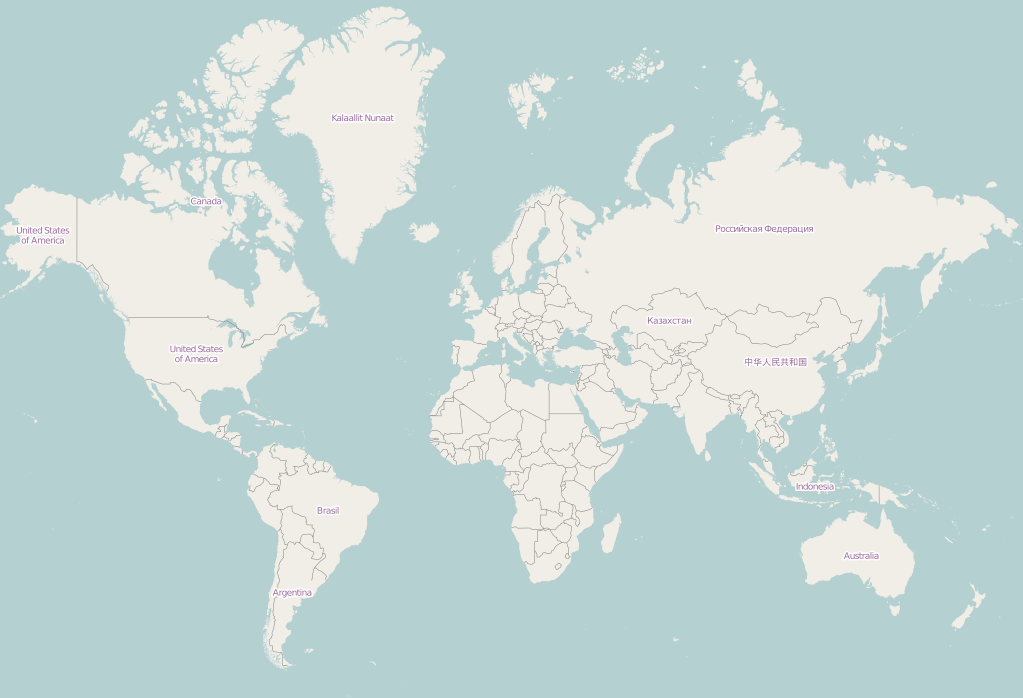
\includegraphics[width=\textwidth]{images/worldMap}

	\tikzboverlay[fill=red!20] at (3,6) {
		\begin{tabular}{l}
			Framework \\
			- module 1 \\
			$ \quad \vdots$\\
			- module n\\
			- module Tom\\
			- module Conny\\
			- module Lara\\
			- module Ben\\
		\end{tabular}
	};
	\tikzoverlay[] at (1,5.5) {
\includegraphics[scale=0.1]{images/smiley}};
	\tikzoverlay[] at (7.5,6) {
\includegraphics[scale=0.1]{images/smiley}};
	\tikzoverlay[] at (8.3,2.5) {
\includegraphics[scale=0.1]{images/smiley}};
	\tikzoverlay[] at (3,7) {
\includegraphics[scale=0.1]{images/smiley}};
	\tikzoverlay[] at (0.3,5.8) {Conny};
	\tikzoverlay[] at (6.9,6.3) {Tom};
	\tikzoverlay[] at (7.8,2.8) {Ben};
	\tikzoverlay[] at (2.4,7.3) {Lara};

\pnote{
	share your modules with other people all around the world\\
	international world wide project
}

\end{frame}

\begin{frame}{Parallel execution}
	\begin{mdframed}[backgroundcolor=orange!40]
		\begin{center}
		\begin{tikzpicture}[node distance=1.5cm]
			\node[draw,rectangle,rounded corners] (st1) {step 1};
			\node<1>[draw,rectangle,rounded corners] (st3) [below of=st1] {step 3};
			\node<2>[fill=yellow, draw,rectangle,rounded corners] (st3) [below of=st1] {step 3};
			\node<1>[draw,rectangle,rounded corners] (st2) [left of=st3] {step 2};
			\node<2>[fill=yellow,draw,rectangle,rounded corners] (st2) [left of=st3] {step 2};
			\node<1>[draw,rectangle,rounded corners] (st4) [right of=st3] {step 4};
			\node<2>[fill=gray!20,draw,rectangle,rounded corners] (st4) [right of=st3] {step 4};
			\node<1>[draw,rectangle,rounded corners] (st6) [below of=st4] {step 6};
			\node<2>[fill=gray!20,draw,rectangle,rounded corners] (st6) [below of=st4] {step 6};
			\node<1>[draw,rectangle,rounded corners] (st5) [left of=st6] {step 5};
			\node<2>[fill=yellow,draw,rectangle,rounded corners] (st5) [left of=st6] {step 5};
			\node[draw,rectangle,rounded corners] (st7) [below of=st5] {step 7};
			\draw [thick,->] (st1) -- (st2);
			\draw [thick,->] (st1) -- (st3);
			\draw [thick,->] (st1) -- (st4);
			\draw [thick,->] (st2) -- (st5);
			\draw [thick,->] (st3) -- (st5);
			\draw [thick,->] (st4) -- (st6);
			\draw [thick,->] (st5) -- (st7);
			\draw [thick,->] (st6) -- (st7);
		\end{tikzpicture}
		\end{center}
	\end{mdframed}

\pnote{
	feature in work:\\
	framework finds for itself out which steps can be done in parallel\\
	uses different threads
}
\end{frame}

\begin{frame}{Platform independent}
	\tikzoverlay[] at (0,2.5) {
\includegraphics[scale=0.1]{images/linux}};
	\tikzoverlay[] at (8,2.5) {
\includegraphics[scale=0.1]{images/mac}};
	\tikzoverlay at (3.3,-1) {Microsoft Windows};
	\tikzboverlay[fill=red!20] at (3.7,1) {Framework};


\pnote{
	programmed by using cmake\\
	should work platform independent\\
	unfortunatelly all of us worked on lunux\\
	didnt tested
}

\end{frame}

%%%%%%%%%%%%%%%%%%%%%%%%%%% part 2:  Carsten %%%%%%%%%%%%%%%%%%%%%%%%%%%%%%%%%%%%%%%%%%%%%%%%%%%%%%

\section{Working with the program}
\subsection{User Interfaces}
\begin{frame}[t]{User Interfaces}

	\begin{columns}
		\begin{column}[t]{.5\textwidth}
			\begin{center}
			{\Large GUI}
			\vspace{.5cm}

			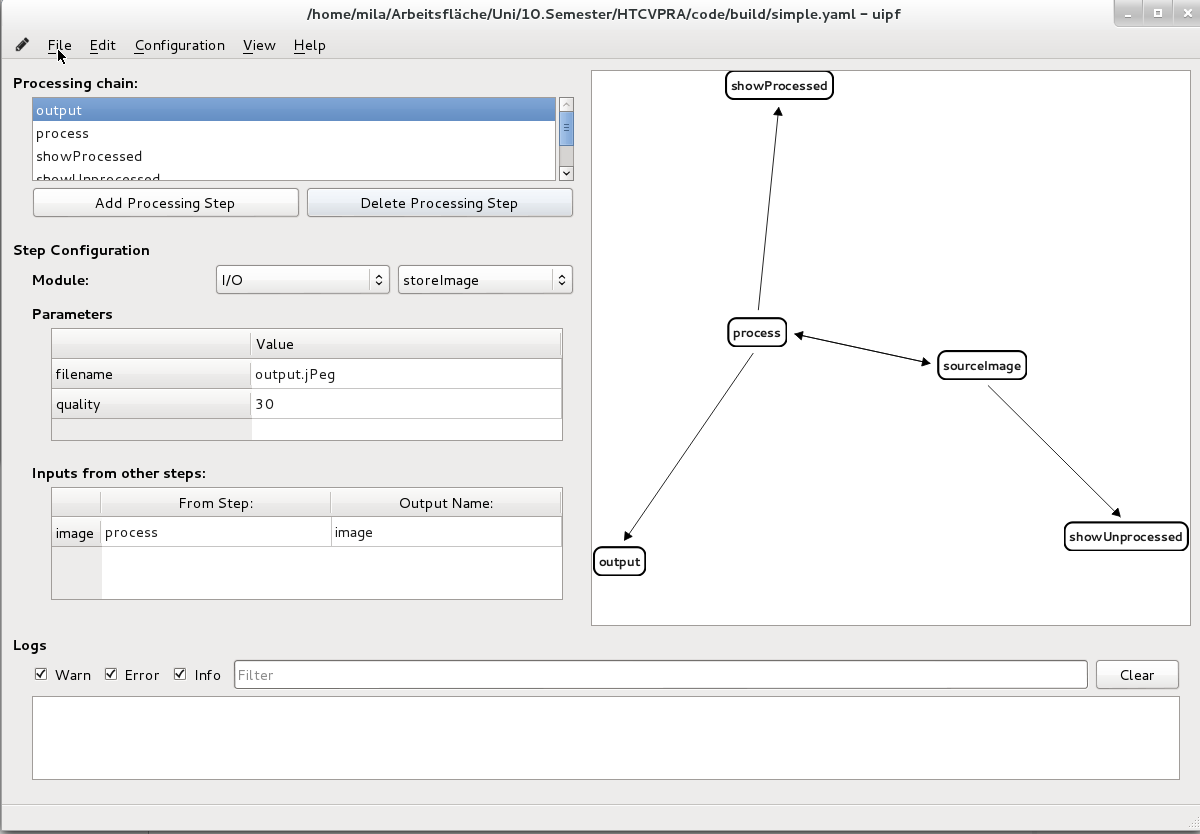
\includegraphics[width=\textwidth]{images/howto/gui}

			\end{center}
		\end{column}
		\begin{column}[t]{.5\textwidth}
			\begin{center}
			{\Large Console}
			\vspace{.5cm}

			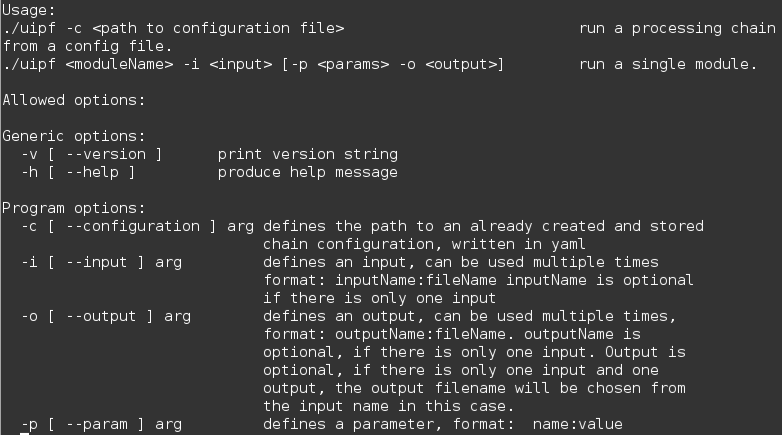
\includegraphics[width=\textwidth]{images/howto/console}

			\end{center}
		\end{column}
	\end{columns}

	\pnote{
		framework provides two interfaces: GUI, Console

		these share a common file format in YAML.

		GUI can create and run chains.

		Console can run a chain and also run single modules.
	}

\end{frame}

\subsection{General Concepts}
\begin{frame}{General Concepts}

	\begin{columns}
		\begin{column}[t]{.4\textwidth}
\Large
			Processing Chain
			\vspace{.4cm}\pause
\Large
			\begin{itemize}
				\item<2->[$\rightarrow$] Processing Step
				\vspace{.25cm}
				\large
				\begin{itemize}
					\item<3->[$\rightarrow$] Module
				\vspace{.25cm}
					\item<4->[$\rightarrow$] Parameters
				\vspace{.25cm}
					\item<5->[$\rightarrow$] Dependencies
				\end{itemize}
			\end{itemize}

		\end{column}
		\begin{column}[t]{.6\textwidth}
			\begin{center}

				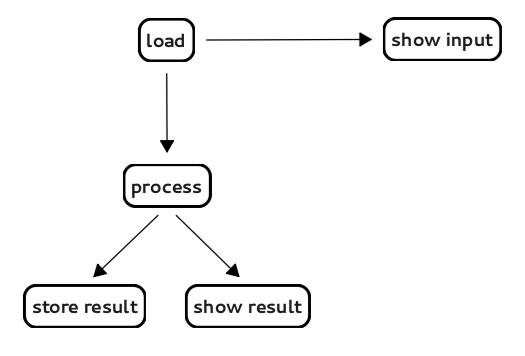
\includegraphics[width=\textwidth]{images/intro/simpleChain}

			\end{center}
		\end{column}
	\end{columns}

	\pnote{
		Processing chain consists of processing steps

		step has a module: e.g. load, store, show, gauss, ...
		+ parameters

		data flow is described using dependencies

		input of one module is the output of another
	}

\end{frame}

\subsection{Storage format}
\begin{frame}[fragile]{Storage format: YAML}

	\begin{columns}
		\begin{column}[t]{.7\textwidth}

			\begin{linehighlight}{
				\only<2>{ \highline{1,5,12} }
				\only<3>{ \highline{2,6,13} }
				\only<4>{ \highline{3,9,10} }
				\only<5>{ \highline{7,8} }
				\only<6>{ \highline{14,15} }
			}
				\lstset{language=yaml}
				\lstinputlisting{images/howto/format.yaml}
			\end{linehighlight}

		\end{column}
		\begin{column}[t]{.3\textwidth}
			\begin{center}

				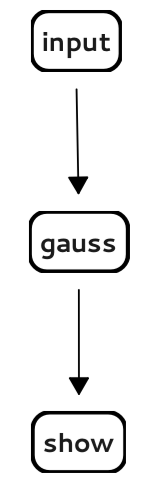
\includegraphics[height=5cm]{images/howto/format.png}

			\end{center}
		\end{column}
	\end{columns}

	\pnote{
		human readyble format\\

		indentation is important!\\
		yaml file shows a map  key => value

		1. each step has a name

		2. has a module

		3. has params to describe behavior of the module

		4. input refers to the step it depends on\\
			can have multiple\\
			refers to image output of the input step\\

		5. same for show, refers to image output of gauss step
	}

\end{frame}

\subsection{GUI}
\begin{frame}{The Graphical User Interface}

\only<1,3>{
	\begin{center}
	\makebox[\textwidth]{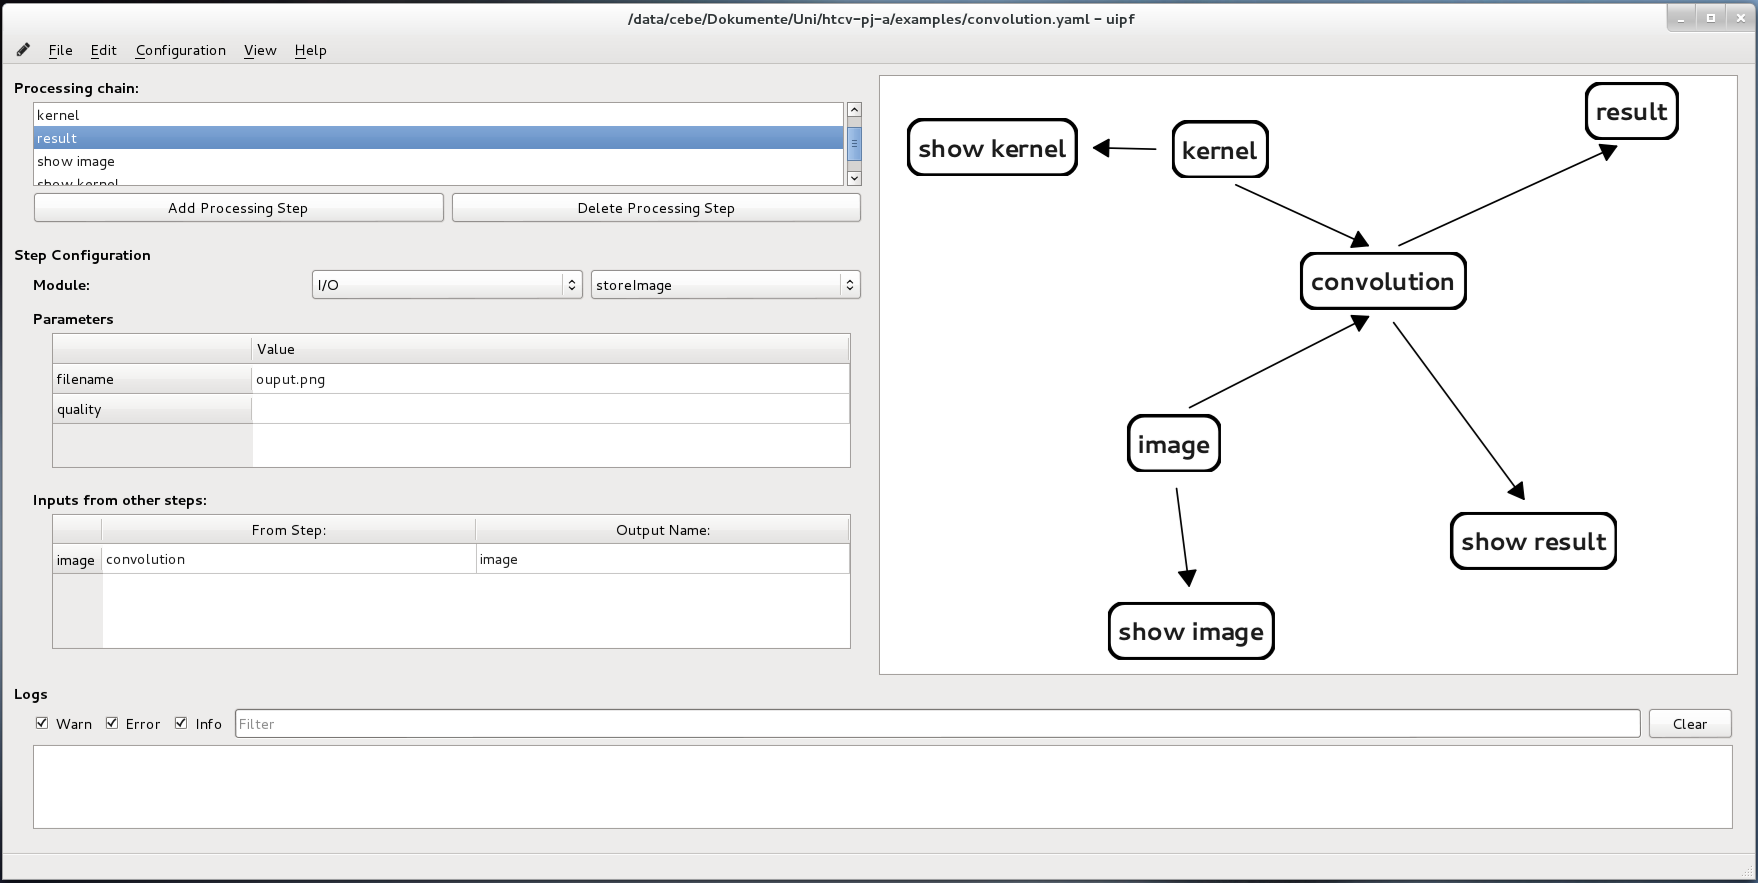
\includegraphics[width=\paperwidth]{images/howto/guiexample}}
	\end{center}
}
\only<2>{
	\begin{center}
	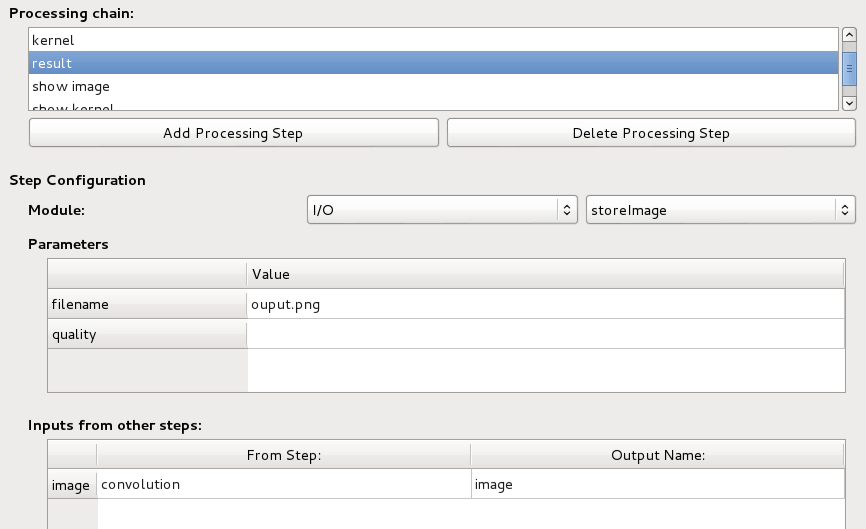
\includegraphics[height=6cm]{images/howto/stepconfig}
	\end{center}
}
	\pnote{
		left: chain config

		right: visualization of the dataflow

		bottom logs, and progress info
	}

\end{frame}

\begin{frame}{The Graphical User Interface}
	\begin{center}
	\makebox[\textwidth]{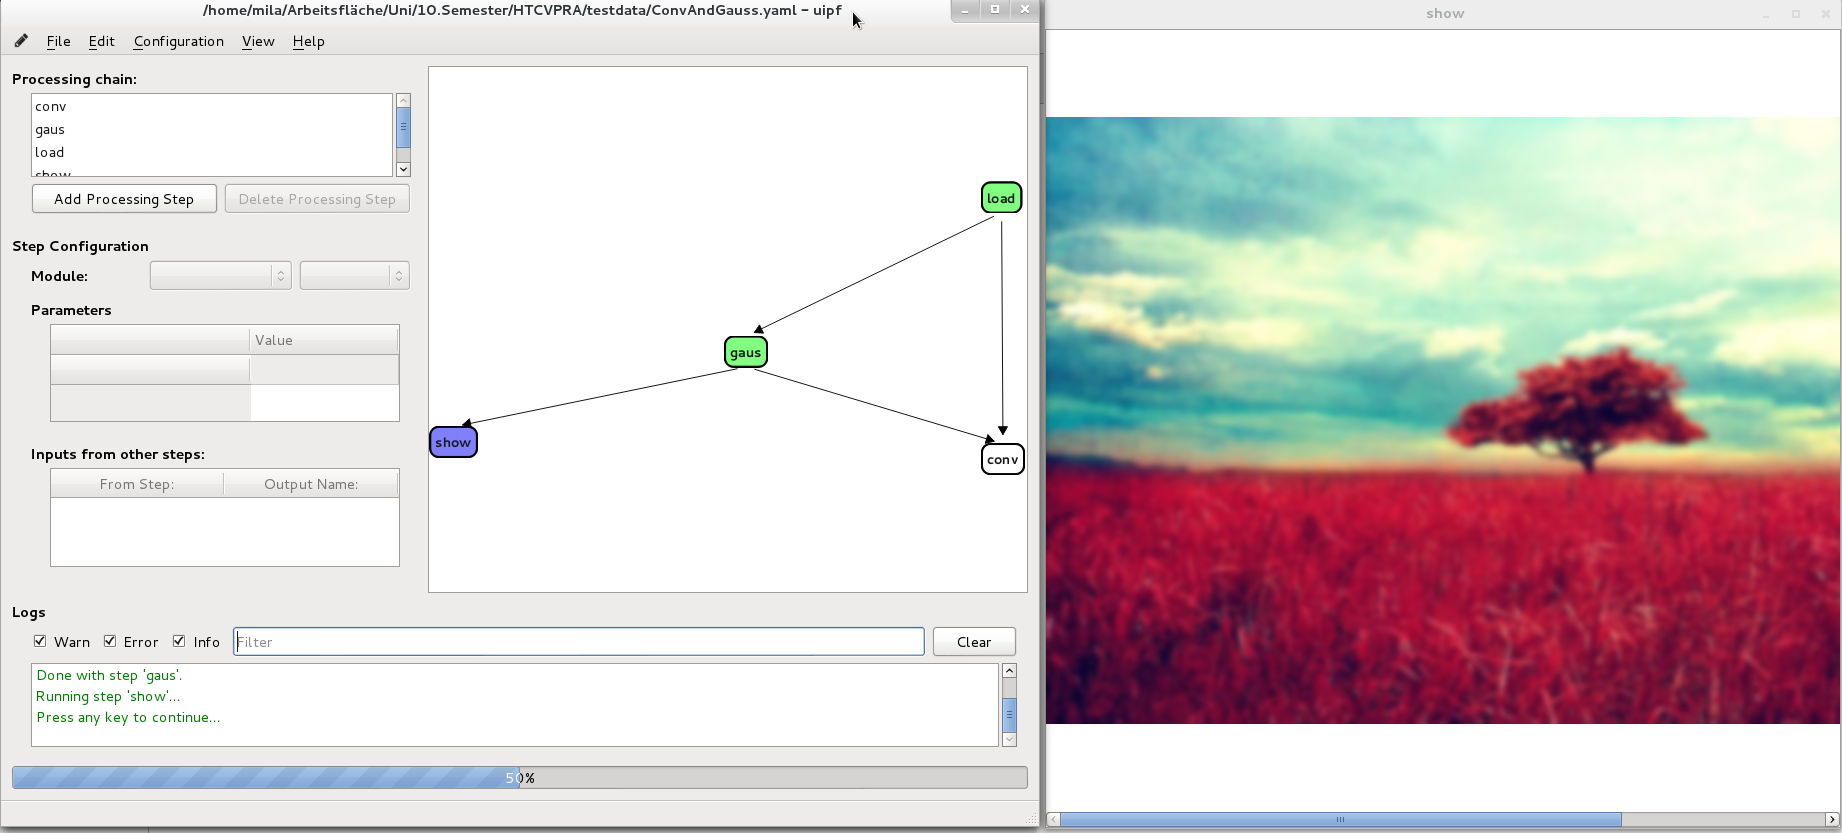
\includegraphics[width=\paperwidth]{images/runChain}}
	\end{center}
\end{frame}

\begin{frame}{The Graphical User Interface}
	\vspace{-.3cm}
	\begin{center}
	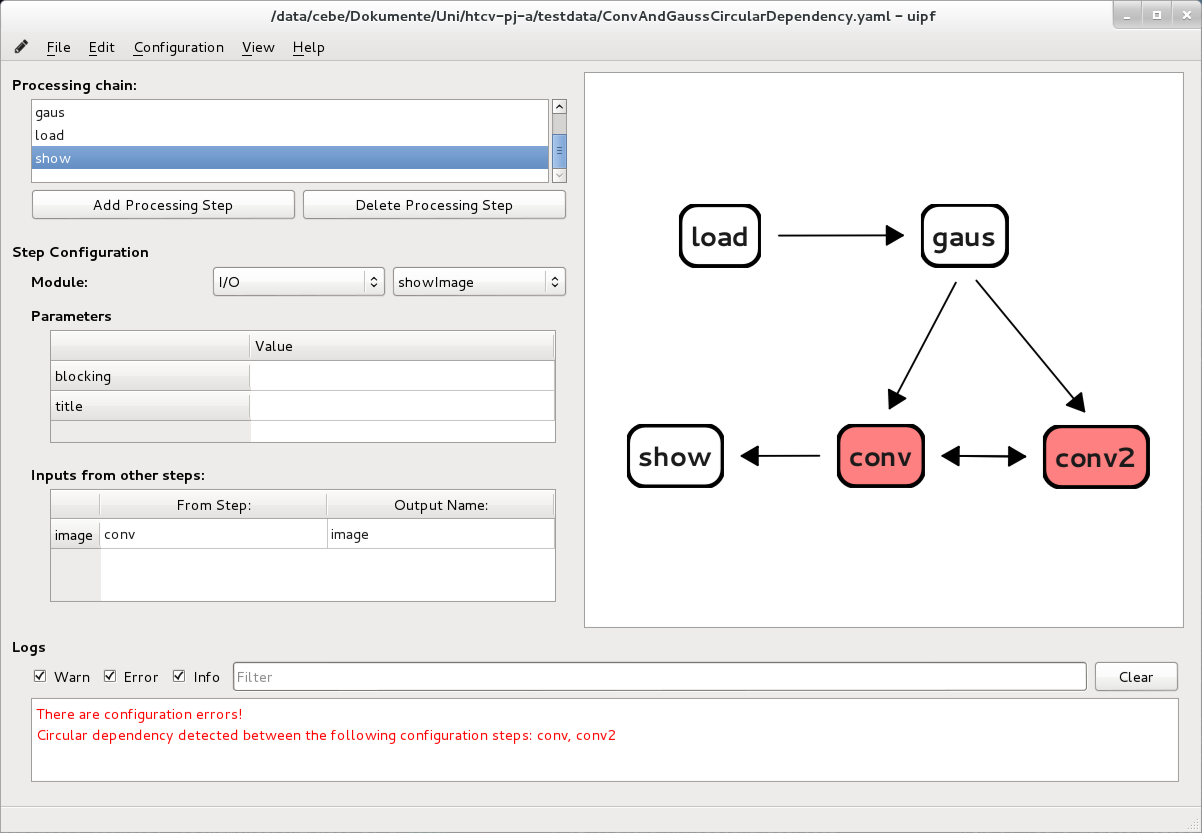
\includegraphics[width=.9\textwidth]{images/howto/errors}
	\end{center}

	\pnote{
		open an existing chain\\
		run/stop the chain\\
		create a new chain/modify existing chain\\
		save the chain\\
		run a buggy chain
	}

\end{frame}

\begin{frame}{Interface features: Graph}
	\begin{center}
	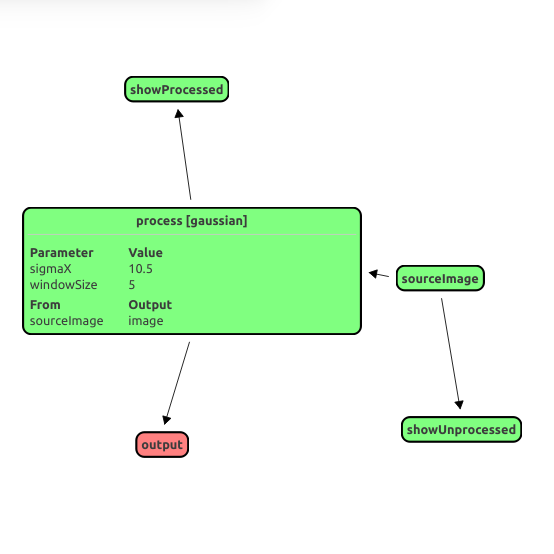
\includegraphics[scale=0.4]{images/graph}
	\end{center}
	\pnote{
		 automatic layout of processing graph

		 simple- and detailview

		 synchronized with current step

		 color coded errors and executionsteps

		 zoom, autoscale and user dragable
	}

\end{frame}

\subsection{Console}
\begin{frame}{The Console Interface}
\Large
\pnote{	Run a processing chain from a config file}

	{\tt ./uipf -c myconfig.yaml}
\pause

	\vspace{.5cm}

\pnote{	Run a single module:

usefule to test different params

run an opencv function just right on a file w/o writing any code
}

	\begin{align*}
		\texttt{ ./uipf <moduleName>} & \texttt{ -i <input> } \qquad \qquad \qquad \\
									  & \texttt{ -p <params>} \dots \\
									  & \texttt{ -o <output>}
	\end{align*}


\end{frame}

\begin{frame}{The Console Interface}
\Large
	\begin{align*}
		\texttt{./uipf gaussian} & \texttt{ -i input.jpg -p sigmaX:5} \\
	\end{align*}
	\vspace{-1.5cm}\pause
	\begin{align*}
		\texttt{./uipf gaussian} & \texttt{ -i input.jpg -p sigmaX:5} \\
								 & \texttt{ -o notdefault.png}\\
	\end{align*}
	\vspace{-1.5cm}\pause
	\begin{align*}
		\texttt{./uipf convolution} & \texttt{ -i image:input.jpg} \\
									& \texttt{ -i kernel:kernel.png} \\
									& \texttt{ -p sigmaX:5 -o out.png}
	\end{align*}

\end{frame}


%%%%%%%%%%%%%%%%%%%%%%%%%%% part 3  Marcus %%%%%%%%%%%%%%%%%%%%%%%%%%%%%%%%%%%%%%%%%%%%%%%%%%%%%%

\section{How to write a new module}

\subsection{What is a module}
\begin{frame}[fragile]{Basics}

Modules are precompiled extensions that:
	\begin{itemize}
		\item encapsulate functionality which can be used in processingsteps
		\item are binary files, shareable without sourcecode (QTPlugin)
		\item implement a simple interface
		\item can include own libs as they need them
		\item have Metadata displayed in the GUI
	\end{itemize}

\end{frame}

\begin{frame}[fragile]{Interface}



	Basic interface: \newline

	\begin{lstlisting}
		string name();
		void run(DataManager& data);
		MetaData getMetaData();
	\end{lstlisting} \pause

 	MetaData: \newline

	\begin{lstlisting}
		string, // general verbal description of the module
		string, // category
		DataDescriptionMap, // input
		DataDescriptionMap, // output
		ParamDescriptionMap // params
	\end{lstlisting}


	\pnote{
	}

\end{frame}

\begin{frame}[fragile]{run() method}

	\begin{lstlisting}<1>
void LoadImageModule::run( DataManager& data) const
{
	// (1) get inputs and params:
	//     - data.getInputData(inputName)
	//     - data.getParam (paramName, dafaultValue)
	// (2) work with them
	// (3) create output:
	//     - data.setOutputData(outputName, outputContent);
}
	\end{lstlisting}

\end{frame}


\begin{frame}[fragile]{getMetaData() method}

\begin{linehighlight}{
%      \only<1,3>{ % Only on slides 1 and 3 (beamer stuff)
%            \highline{1,3,5} % highlight code lines 1,3 and 5.
%      }
%      \only<2>{ % Only on slide 2 (beamer)
%            \highline{2,...,8} % highlight lines 2 to 8.
%      }
}
      \lstinputlisting{metadata.cpp}
\end{linehighlight}

\end{frame}


\begin{frame}[fragile]{CMake}

Modules need to be registered in CMakeList.txt: \newline

	\begin{lstlisting}<1>
...
#Image Processing
#ResizeModule
add_library(ResizeModule SHARED modules/improc/ResizeModule.cpp)
qt5_use_modules(ResizeModule Core ) #QtCore is needed for <QPlugin>
target_link_libraries(ResizeModule opencv_core opencv_imgproc ModuleBase)
...
	\end{lstlisting}


	\pnote{
	}

\end{frame}

\begin{frame}[fragile]{Implementation summary}

Steps to create your own Module:
	\begin{enumerate}
		\item Copy .hpp and .cpp of an existing module e.g. the DummyModule \pause
		\item Replace "DummyModule" with your new name \pause
		\item implement your logic in run()  \pause
		\item define your module's metadata \pause
		\item edit CMakeList.txt \pause
		\item run make
	\end{enumerate}


	\pnote{
	}

\end{frame}


%%%%%%%%%%%%%%%%%%%%%%%%%%% part 4:  Akarsh %%%%%%%%%%%%%%%%%%%%%%%%%%%%%%%%%%%%%%%%%%%%%%%%%%%%%%

%~ \section{Testing}
%~ \begin{frame}{run with TestRail}
	%~ 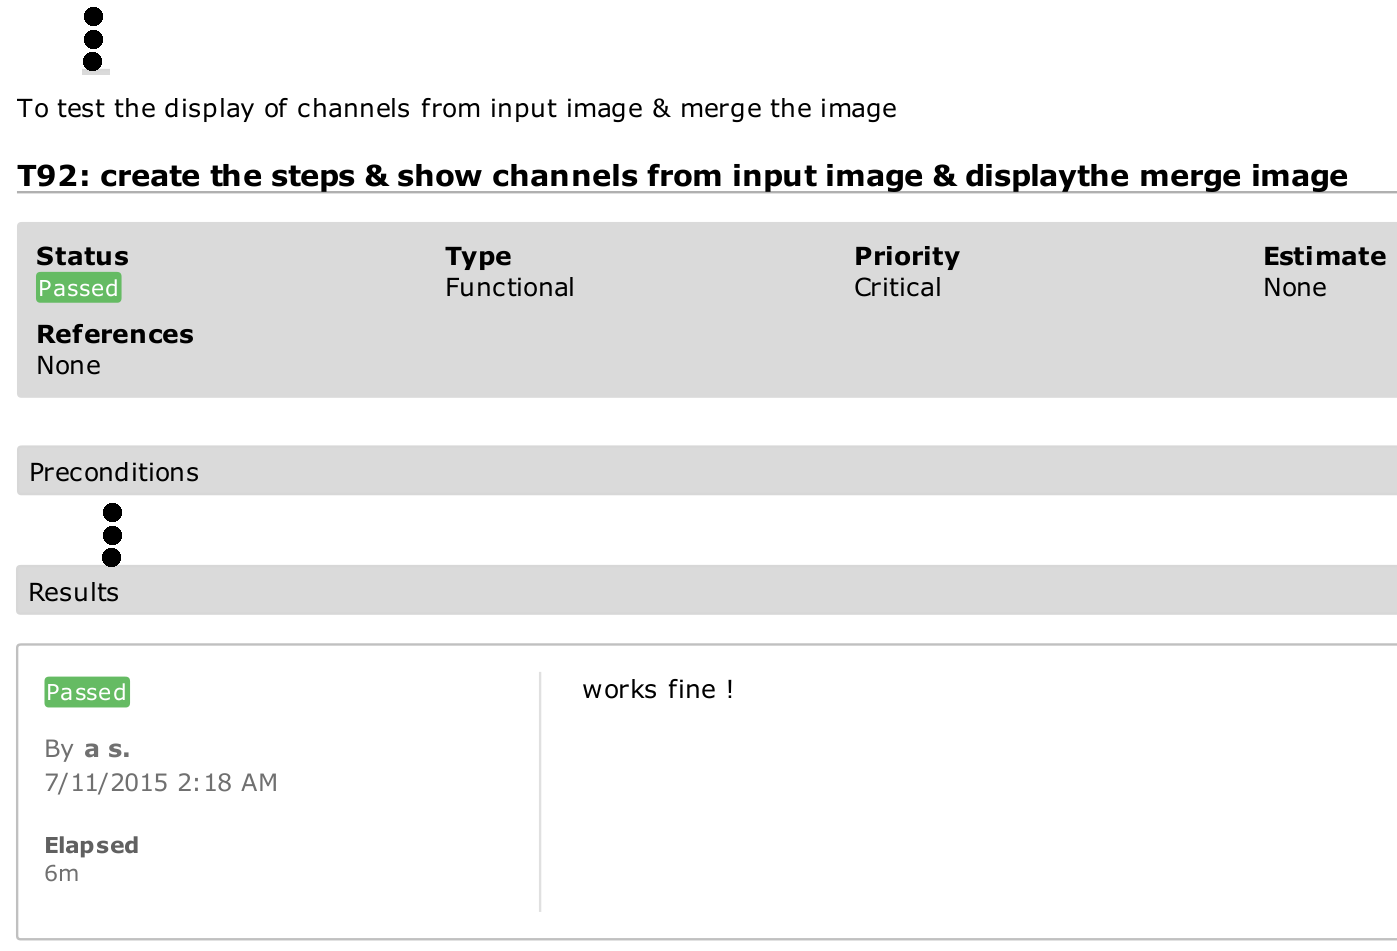
\includegraphics[width=\textwidth]{images/eval}
%~ \end{frame}
%~
%~ \begin{frame}{Video Tutorial}
%~ \end{frame}


%%%%%%%%%%%%%%%%%%%%%%%%%%% part 5:  All of us %%%%%%%%%%%%%%%%%%%%%%%%%%%%%%%%%%%%%%%%%%%%%%%%%%%%%%

\section{Live Demo}

\begin{frame}{Live Demo}

\begin{center}
	{\Huge
	Live Demo!}
	\vspace{2cm}

	Fork us on Github:\\\vspace{0.2cm}
	\url{https://github.com/TU-Berlin-CVRS/uipf}

	\pnote{
		first: Questions?\\
		We are on github!\\
		second: Live Demo.
	}
\end{center}
\end{frame}

\end{document}
